%%
%% VERSION HISTORY
%%    22 May 2006 - John Papandriopoulos - Original version
%%    12 Jul 2007 - John Papandriopoulos - Converted into template
%%

\chapter{Tools and resources}
	\label{chapter:empire-strikes-back}%
	%

% preferred location for figures in this chapter
\setfigurepath{figures/chapter-3}

%=========================================================================

%=========================================================================
\section{Framework and libraries}
\subsection{NLTK}
NLTK\footnote{http://www.nltk.org/} (\textbf{N}atural \textbf{L}anguage \textbf{T}ool\textbf{K}it) is a popular framework for working with human language. It is developed by Steven Bird\footnote{http://www.stevenbird.net/}, Ewan Klein\footnote{http://homepages.inf.ed.ac.uk/ewan/} and Edward Loper\footnote{http://ed.loper.org/}. The project was started in 2001 and still continue to update and release at the time of writing. The platform provides a suite of processing libraries for text classification, stemming, tokenization, parsing, tagging and semantic reasoning functionalities. It also serve as wrappers for other NLP libraries such as Stanford CoreNLP \cite{manning-EtAl:2014:P14-5}. We can easily access more than 50 corpora and other lexical resources such as WordNet\textsuperscript{\textregistered} through interfaces of Python programming language.\\
Authors of NLTK also published the book \textit{Natural Language Processing with Python} \cite{Bird2009} to give practical introduction and hands-on guide to programming for NLP. The book covers many topics of computational linguistic, their examples by graphical demonstrations and sample data. Along with comprehensive online documentation, readers learn the fundamentals of writing Python scripts for NLP tasks like categorizing text, working with corpora and analyzing linguistic structure of them. Both NLTK and the book are free of charge and publicly available online. As a result, NLTK is used as a teaching tool for NLP education in many universities around the world.\\

\subsection{Scikit-learn}
Scikit-learn\footnote{http://scikit-learn.org/} is a free software package for machine learning and data analysis written in Python \cite{scikit-learn}. The project was originally started in 2007 by David Cournapeau\footnote{https://github.com/cournape} and still under active development as of 2017 by many different researchers and developers. Like NLTK, scikit-learn is designed for Python and compatible with other numerical and scientific Python libraries like NumPy and SciPy. Scikit-learn features machine learning algorithms for classification, clustering and regression tasks such as linear regression, SVM, k-means, decision tree and boosting. It is very well-maintained with stable release and online documentation on its website. Furthermore, each algorithm and its variant are illustrated by practical examples including brief explanation with citation, figures and sample code with comments to enhance readers' understanding of the problem. 


\section{Employed NLP methods}
\subsection{Tokenization}
\textit{Tokenization} is usually a crucial step appearing in early stage of the NLP workflow to facilitate processing with more complex analytical techniques. Tokenization is the task of divide a character sequence into defined document units referred as tokens. A token is defined as "an instance of a sequence of characters in some particular document that are grouped together as a useful semantic unit for processing" \cite{Manning:2008:IIR:1394399}. In theory, tokens can take form of any textual elements of chosen granularity such as punctuation or fomulae but in practice, tokens are usually words.\\

\begin{figure}
\centering
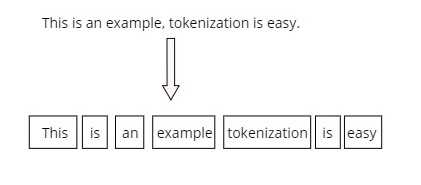
\includegraphics[width=\textwidth, clip=true, height = 5.5cm]{img/tokenization_example}
\caption[Tokenization example]{ Example of tokenization. Tokenizer splits a sentence into words.} 
\label{fig:token_ex1}
\end{figure}

As shown in Figure~\ref{fig:token_ex1}, tokenization have dropped punctuation of the sentence and each word is getting full meaning. However, tokenization phase may encounters difficult choice in a broader context. For example, take a look at the sentence "\textit{Tokenization isn't easy}". Two words \framebox{Tokenization} and \framebox{easy} are pretty straightforward since they are splitted by whitespace. In contrast, \textit{isn't} can be tokenized by different rules: \framebox{isn't}, \framebox{isnt}, \framebox{is} \framebox{n't}, \framebox{isn} \framebox{t}. Furthermore, each language and topic contain jargon and words refer to specific entities but are not in standard dictionary. For instance, AK-47 is name of a semi-automatic rifle, programming language C\# and so on. Computer era brings new types of technology terminology, which appear frequently on online document, such as website addresses (https://www.google.com/), email addresses (johndoe@gmail.com), decimal IP addresses (123.172.2.1). These character sequences should be recognized as one entity but in some cases, it would cause unnecessary index to be included in the extracted dictionary. In the experiment of this thesis, NLTK Tokenizer package, which is improved TreebankWordTokenizer \footnote{http://www.nltk.org/api/nltk.tokenize.html\#nltk.tokenize.treebank.TreebankWordTokenizer} along with PunktSentenceTokenizer\footnote{http://www.nltk.org/api/nltk.tokenize.html\#nltk.tokenize.punkt.PunktSentenceTokenizer} for the specified language, was used.\\

\subsection{Stop words removal}
\textit{Stop words} are words that contribute very little in term of semantic, thus being considered low value in IR systems. These words usually appear with high frequency in collection. To remove stop words, high use words must be manually assessed for semantic content. If a word is identify as a stop word, it is added to a list called \textit{stop list}. The length of a stop list varies between less than twenty (15-18 terms) to a few hundred words (200-300 terms). Depending on purpose and scale of a system, a stop list can be very general or specifically relate to a topic.\\
Using a stop list can potentially reduce query time due to smaller index of a system. However, web search engines in practice do not use stop lists partially because of immense server clusters behind them generating enormous computing power. \\
Common words belong to world classes article, conjunction, preposition and frequent words like \textit{now} or \textit{very} are included in stop lists. General-purpose stop lists are available online and can be easily incorporated into IR systems. Sometimes removing stop words can be detrimental as vital information may be missed after going through stop list filter (e.g. \textit{"To be or not to be"} is a well-known verse that may get taken out of indexed vocabulary) so utilization of these lists must be carefully examined. In the experiment of this thesis, Stopwords corpus of NLTK was used. It is a corpus containing 2400 stopwords for 11 languages. Stop list for English contain 153 words.\\

\subsection{Part-of-speech tagging}
A Part-of-speech (POS) tag is category of words assigned to a word which display similar (primarily syntactic) grammatical properties of it in the sentence. Words that share the same POS tag 
typically play similar roles in structure of sentences. Example of some POS tags are NOUN (noun), ADJ (adjective), VERB (verb), PRON (pronoun). In practice, there are many sets of POS tag (tagset) such as Universal\footnote{http://universaldependencies.org/u/pos/}, Treebank. Some tagsets usually comprise fine-grained tag like "singular proper noun" for more complex analyzing task. In early years of building automatic POS tagger, handwritten rules distinguish parts of speech much like decision tree. These rules may work in a particular type of document or some set of rules can be applied widely to many text corpora of a language.\\
When machine learning techniques are utilized for POS tagging task, there are three main approaches: statistical tagging, rule-based tagging and hybrid tagging. Statistical tagging relied on corpora annotated by human as training data to compute probability of a specific token belong to a POS tag category. The drawback of statistical tagger is some tagged sequences are not correct due to low usage in a language. In other word, it is susceptible to rare case of word in an unfamiliar context and most of the time misclassify to usual tag of that word. Hybrid approach require both hand coded rules and probabilistic features of words, but it is not widely used in practice since balancing weight between these two features is not an easy task for a general-purpose tagger.\\
\begin{figure}
\centering
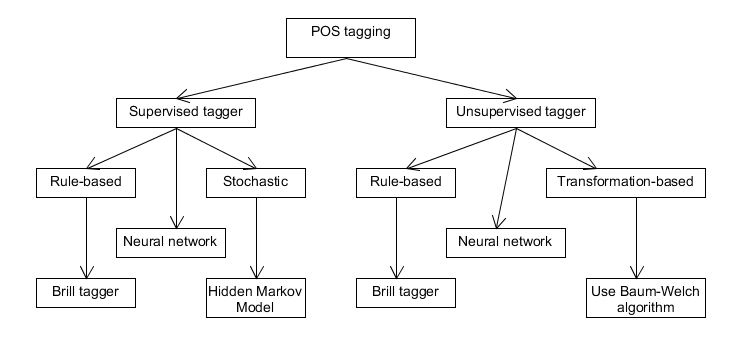
\includegraphics[width=\textwidth, clip=true]{img/POS_tagger}
\caption[POS tagger classification]{POS tagger classification} 
\label{fig:pos_tag}
\end{figure}
Figure~\ref{fig:pos_tag} shows classification of POS tagger. Neural network, rule-based tagger can be either supervised or unsupervised learning paradigm. POS tagging plays an important role in the experiment of this thesis as we need to extract tags like nouns, verbs, adverbs. In the experiment, we used NLTK POS tagger which is a neural network tagger trained on Penn TreeBank corpus.
\subsection*{Sentiment analysis}
Sentiment analysis is the process of identifying, quantifying the sentiment content of a text using NLP or statistical methods. The general approach is to enumerate words that express emotions, opinions, attitudes and assign scores to them. There are several prominent lexicons for sentiment analysis such as LIWC, SentiWordNet, SenticNet\footnote{http://sentic.net/}, VADER\footnote{https://github.com/cjhutto/vaderSentiment}. The lexicon we chose is VADER (\textbf{V}alence \textbf{A}ware \textbf{D}ictionary and s\textbf{E}ntiment \textbf{R}easoner). VADER is a simple rule-based model built on lexical features which are attuned to sentiments expressed in social media context \cite{Hutto2014}. VADER returned four types of scores for each sentence: positive, negative, neutral and compound. The first three scores are proportions of text that fall in each corresponding category thus they are add up to 1. The compound score is in interval [-1, 1] with -1 indicates extreme negative and 1 indicates extreme positive.\\

\section{Employed ML models}
We use three off-the-shelf models offered in scikit-learn for the experiment of this thesis.
\subsection{Na\"ive Bayes}
Na\"ive Bayes is a probabilistic model based on Bayes' theorem. It assumes features are independent from each other. Given a feature vector $\textbf{x} = (x_1, x_2,..., x_2)$ representing $n$ independent variables and a target class variable $y$, the conditional probability of instance $\textbf{x}$ belong to class $y$ can be expressed as:
\begin{eqnarray*}
P(y | x_1, x_2,..., x_n) = \frac{P(y)P( x_1, x_2,..., x_n | y)}{P( x_1, x_2,..., x_n)}
\end{eqnarray*} 
The "na\"ive" assumption states that each feature is conditionally independent from every other features: 
\begin{eqnarray*}
P(x_i | y, x_1, x_2,..., x_{i-1}, x_{i+1},...,x_n) = P(x_i | y)
\end{eqnarray*} 
Now, the original probability is simplified:
\begin{eqnarray*}
P(y | x_1, x_2,..., x_n) = \frac{P(y)\prod\limits_{i=1}^n P( x_i| y)}{P( x_1, x_2,..., x_n)}
\end{eqnarray*} 
The classification rule is:
\begin{eqnarray*}
P(y | x_1, x_2,..., x_n) \propto P(y) \prod\limits_{i=1}^n P( x_i| y)\\
\Rightarrow\hat{y} = \argmax_y P(y)  \prod\limits_{i=1}^n P( x_i| y)
\end{eqnarray*}
where $\hat{y}$ denotes the prediction outcome.

\subsection{Logistic regression}
Logistic regression is regression model that is widely used in binary classification task (the dependent variable takes only two values). Logistic regression is one of linear models where the response (dependent) variable is estimated using linear function:
\begin{eqnarray*}
y = w_0 + w_1x_1 + ... + w_nx_n
\end{eqnarray*}
Weights and features can be represented in vector form $\textbf{w} = (w_1, w_2,...,w_n)$ and $\textbf{x} = (x_1, x_2,...,x_n)$. The probability function estimating likelihood of $y$ belong to positive class ($y = 1$) is:
\begin{eqnarray*}
P(y = 1 | \textbf{x}) = \frac{1}{1+exp(-\textbf{w}^\intercal\textbf{x})} = \sigma(\textbf{w}^\intercal\textbf{x})
\end{eqnarray*}
where $\sigma(z) = \frac{1}{1 + exp(-z)}$ is called \textit{sigmoid} or \textit{logistic} function.

\subsection{Support vector machines}
Support vector machines is a set of supervised learning models used for classification and regression task. In general, SVM try to establish one or more hyperplane to separate data points and assign them to target classes. Suppose we have a training dataset $(\vec{\bm{x}}_1, y_1), (\vec{\bm{x}}_2, y_2),...,(\vec{\bm{x}}_n, y_n)$ where $y$ either take values -1 or 1 (binary case) and $\vec{\bm{x}}_i$ is a feature vector. A hyperplane can be represented as:
\begin{eqnarray*}
\vec{\bm{w}} . \vec{\bm{x}} - b = 0
\end{eqnarray*}
where $\vec{\bm{w}}$ is the normal vector to the hyperplane. If data points are linearly separable, we want to maximum distance between two classes. We define two hyperplanes $\vec{\bm{w}} . \vec{\bm{x}} - b = 1$ and $\vec{\bm{w}} . \vec{\bm{x}} - b = -1$. The distance between them is $\frac{2}{||\textbf{w}||}$ where $||\textbf{w}|| = \sqrt{w_1, w_2,...,w_2}$.\\
Our objective is to maximize
\begin{eqnarray*}
\min_{i = 1,\dots,n} = \frac{y_i(\vec{\bm{\textbf{w}}} . \vec{\bm{\textbf{x}}}+b)}{||\textbf{w}||}
\end{eqnarray*}
as a function of $\textbf{w}$ and b.\\





